%
% Sample SBC book chapter
%
% This is a public-domain file.
%
% Charset: ISO8859-1 (latin-1) áéíóúç
%
\documentclass{SBCbookchapter}
\usepackage[utf8]{inputenc}
\usepackage[T1]{fontenc}
\usepackage[brazil,english]{babel}
\usepackage{graphicx}
\usepackage{array}

\author{Sam Haynes}
\title{User-Friendly, Open Source Research Software}

\setcounter{chapter}{3}

\begin{document}
\maketitle

\begin{abstract}
This chapter explores the development and improvement of an open source R package called tidyqpcr. The introduction discusses the motivation for creating a package that aids the design, analysis and presentation of qPCR assays. It introduces the growing issue with reproducing results based on qPCR data as well as the benefits of applying experimental design techniques to the planning of qPCR experiments. The decade old best practices for conducting and publishing qPCR experiments, the MIQE- guidelines are introduced. Finally, concerns around the dependence of close source, proprietary and untested Cq calculation algorithms used to across disciplines. Then, the results section first summarises the semi-structured interviews of several experimental biologists to discern current patterns in qPCR assay design and analysis. This provides the framework for a review of currently available software packages for the analysis of qPCR data. The chapter then introduces tidyqpcr and how its functions and detailed vignettes facilitate the block design of qPCR plates. How it integrates into a larger package ecosphere for advanced downstream analysis and outlines a flexible but regular analysis pipeline incorporating key QC steps. Finally, the chapter discusses how user interviews have helped expand and improve tidyqpcr.


\end{abstract}

\section{Chapter 3 Introduction}

\section{Chapter 3 Results}

\subsection{Theme derived from semi-structured interviews}
The six interviewees varied from experienced post-doctoral research assistants to undergraduates with experience in both both programming and conducting qPCR assays varying from novice to expert.
Excel remains a common piece of software for the analysis of qPCR results and design of plates.
The awareness of MIQE guidelines is remains relatively unknown.
Users almost universally depend on qPCR machine software to determine qc values.
Very few interviewees recall published data giving QC results, analysis code or detailed protocols.
Commonly three replicates are used although some users remove outliers but some do not.
Not everyone checks amplification curves or confirms linear efficiency.
Although most users are confident they could re-analysis their own results no-one reported that their analysis was openly available for reviewers to reader to use with requesting access.
Users all reported doing RNA not DNA quantification.
Few had attempted to recreate any other published data set but despite qPCR being considered a "gold standard" in nucleotide quantification a regular theme of not trusting conclusions based on qPCR results alone was common. 
Few were aware of the concept of 'tidy' data outside of users already using R packages  based on the tidyverse.

\begin{figure}[t]

{\centering 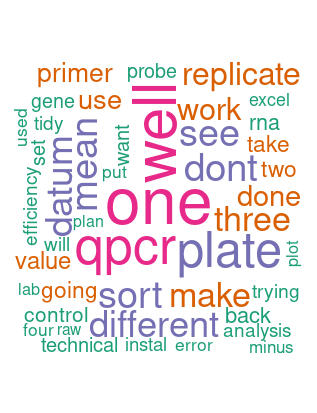
\includegraphics[width=0.5\linewidth]{figures/mg_rb_ck_ec_db_semi_structured_word_cloud} 

}

\caption{\textbf{A text cloud showing the key words repeatedly used across the semi-structured interviews.} The greater the frequency of a word the larger it appears in the figure. }\label{fig:semi-structured-test-cloud}
\end{figure}

qPCR machines are susceptible to multiple systematic biases. Positional effects can be a significant contribution to measured expression. Edge wells may be more likely to have some of their liquid evaporate away. Multichanel pipettes may consistently output lower/higher volumes out of sepcific tips. Thermal gradients may be uneven across the plate. Therefore, grouping biological/technical replicates so they are place in the neighbouring wells could lead to systematic effects confounding biological effects. This can compound even further if the same samples are place in the similar positions across multiple different wells. In an ideal situation, different samples and their replicates should be allocated entirely random well positions. However, if the sample loading is manual then having inconsistent loading plans across plates can lead to incorrect loading; i.e. the wrong sample in the wrong well. Ultimately, having an incorrect map of samples in wells is significantly more detrimental to any analysis than systematic bias. A balance between easy loading and good experimental design principles are required. In tidyqpcr, we have built several plate plan helper functions built around block designs. This enables samples to be spread across the plate and minimise well position biases but still contain regular patterns for loading with multi-channel pipettes. We also describe in detail different plate design strategies than user can explore depending on their particular pipettes and plates. Users can exclude loading samples into edge wells with the provided helper functions. We are also exploring introducing automatic generation of loading recipes for common liquid handlers so users with the access to the appropriate equipment can ensure the loader and plate plan match identically.

% Q. Liu and M. Markatou, 2016, Evaluation of Methods in Removing Batch Effects on RNA-seq Data, Infectious Diseases and Translational Medicine

% Schurch et al, 2016 many replicate RNA sequencing

\subsection{Quantitative PCR}

\subsection{Comparing current qPCR analysis software}

Previous reviews \cite{Rodiger2015, Pabinger2014}

Introducing RDML \cite{Rodiger2017}

%Check for software:
%- plate plan
%- version
%- release
%- missing data interpolation
%- normalisation
%- auto-dection of normalising genes
%- absolute or relative quantification
%- plot melt/amp curves
%- standard / efficiency calcs 
%- efficiency in quant calc
%- statistical analysis
%- plotting results
%- support for taqman probes


\textbf{Web Apps}

\textbf{QuantGenius} A standalone web-app for absolute quantification of target abundance with quality control. The analysis pipeline uses standard curves to determine target abundance, checks copy number and summarises multiple QC steps in the final view to aid users in determining significant results. It uses a PHP backend to conduct the analysis.   \cite{Baebler2017}

\textbf{ELIMU-MDx} Web-based elixer tool for the storage and anlysis of clinical qPCR data. Uses RDML to store qpcr machine agnostic metadata and results. Able to deduce relative and absolute target abundance.  \cite{Krahenbuhl2019}

\textbf{shinyCurves} R Shiny web-based app for assay agnostic detection of COVID-19. Accepts excel spreadsheet inputs from qPCR machines and determines if samples are Positive, Negative or Undetermined depending on user defined thresholds. Users can conduct QC too by viewing melt curve plots and amplification curve plots. \cite{OlaecheaLazaro2021}

\textbf{PIPE-T} An extension to the Galaxy web-based bioinformatics platform released in Oct 2019. PIPE-T provides a Galaxy interface for several R based qPCR analysis packages to enable users to chain multiple analysis steps; missing data interpolation, normalisation, and inferring differential expression, without needing to learn to program in R. Flags Cq values with poor quality. It conducts relative quantification but not absolute quantification. Raw Cq values need to be pre-processed so that each sample/replicate/condition is in a separate tab separated text file.  This tool depends heavily on the R packages HTqPCR, NormqPCR described below. \cite{Zanardi2019}

\textbf{SATqPCR} A standalone web-app. Can use primer efficiency in relative quantification count but does not have the functionality to calculate efficiencies from calibration curves. Cannot visualise melt/amp curves. (Rancurel wt al 2019). Raw Cq values need to be pre-processed so that each gene has its own column and the first column has sample name in specific format. Automatically detects most stable genes to use as normalisation genes. Allows t-test and anova statistical tests. Does not detect outliners or missing data interpolation \cite{Rancurel2019}. Based on an R package RqPCRAnalysis (see below).

\textbf{Auto-qPCR} A standalone web-app with Python back-end for the relative and absolute quantification of qPCR data. Users can download the python code to run the app locally. v1 was released in Aug 2020. (Maussion 2021). Enables user-defined multi-reference gene normalisation, outlier identification and up to 2 way anova (for parametric and non-parametric). Does not calculate efficiency or standard curve. \cite{Maussion2021}

\textbf{Chainy} R Shiny web-based app for the relative quantification of targets with efficiency (can calculate efficiency with raw data). Accepts multiple file formats as input: RDML or vender specific outputs. Automatic selection of reference genes (using NormqPCR). Does not remove outliers or conduct missing data interpolation. Can plot amplification and melt curves. Permutation test to fold change significance. \cite{Mallona2017}

\textbf{R Packages}

\textbf{LEMming} A published R script for the normalisation of qPCR data and detection of differential expression without the use of normalising genes. It proposes a linear error model for qPCR experiments and proposes steps to remove several sources of error by assuming the mean $C_t$ values within samples of similarly treated groups are equal. The script primarily depends on BioConductor ExpressionSets, base R linear regression functions and the limma R package. \cite{Feuer2015}

\textbf{pcr} An R package for the quantification of relative transcript abundance. Expects a table of Cq values with each row a different sample as input. Includes functions to conduct statistical tests from t-test to multiple linear regression, normalises to one reference gene. Contains functions to calculate efficiency and the standard curve. \cite{Ahmed2018}

\textbf{HTqPCR} R Bioconductor package for the relative quantification of qPCR data using S4 classes. Input is Cq across genes with each condition contained in separate tab-separated files. User can define outliers of replicates. No automatic reference gene selection but quantile means can be used. Does not plot melt/amp curves. Can test significance with linear models or t-tests. \cite{Dvinge2009}

\textbf{NormqPCR}  R Bioconductor package for the relative quantification of qPCR data using S4 classes. Encapusalates the geNorm function widely used to select reference genes with steady expression. Outliers removed with manual thresholds. Cannot plot melt/amp curves. \cite{Perkins2012}

\textbf{qpcR} An R package for selecting the best sigmoidal model to fit to qPCR data for accurate determination of Cq values and PCR efficiency. It can detect sample outliers. It does not calculate relative or absolute abundances or conduct any significance analysis. \cite{Ritz2008}

\textbf{Misc}

\textbf{Spreadsheet} Published guide for determining relative abundance using spreadsheet software. It provides steps starting from importing qpcr machine data determining significant differential expression. It does not include quality control measure or removal of outliers. \cite{Ng2021}

\subsection{tidyqpcr}

Our package, tidyqpcr, addresses the need for a qPCR analysis package that fully integrates with the user-friendly tidyverse, encourages the use of MIQE best-practice compliant experimental design, and provides detailed example analysis pipelines as R vignettes. Following the tidy data paradigm integrates tidyqpcr into the wider collection of data analysis packages provided by the tidyverse, while being accessible to novice users of R. Other open-source libraries for qPCR analysis are available with distinct aims. HTqPCR [@Dvinge:2009], ReadqPCR/NormqPCR [@Perkins:2012], and qpcR [@Spiess:2018] have similar and in some respects greater functionality than tidyqpcr, but follow object oriented approaches with specialised data objects. By contrast, pcr [@Ahmed:2018] aligns most closely with tidyqpcr but its function inputs are not tidy data frames. Although alternatives are available, tidyqpcr's aims and approach are distinct: to improve the quality of qPCR experiments from plate design to analysis, by exposing all data in a consistent tidy format that integrates with the tidyverse.

\subsubsection{tidyqpcr aims}

\begin{itemize}
    \item Empowering: tidyqpcr combines a free, open-source qPCR analysis R package with online teaching materials.
    \item Reproducible: tidyqpcr scripts produce paper-ready figures straight from raw data with identical results across computers.
    \item Flexible: tidyqpcr follows the 'tidy' data paradigm to ensure scalability and adaptability.
    \item Best-practice compliant: tidyqpcr encourages standardised, reliable experimental design by prioritising MIQE-compliant best practices.
\end{itemize}

\subsubsection{tidyqpcr functionality}

tidyqpcr can be used to analyse qPCR data from any nucleic acid source - DNA for qPCR or ChIP-qPCR, RNA for RT-qPCR. Currently tidyqpcr has functions that explicitly support relative quantification by the $\Delta Cq$ method, but not yet absolute quantification.

\begin{itemize}
    \item use a single data type for analysis as every object is a tibble / data frame.
    \item lay out and display 96/384-well plates for easy experimental setup (label\_plate\_rowcol, create\_blank\_plate, ...).
    \item consistently describe samples and target amplicons with reserved variable names (sample\_id, target\_id).
    \item flexibly assign metadata to samples for visualisation with ggplot2 (see vignettes).
    \item read in quantification cycle (Cq) and raw data from Roche LightCycler machines with single-channel fluorescence (read\_lightcycler\_1colour\_cq, read\_lightcycler\_1colour\_raw).
    \item calibrate primer sets including estimating efficiencies and visualization of curves (calculate\_efficiency).
    \item visualize amplification and melt curves (calculate\_drdt\_plate)
    \item perform normalisation and relative quantification to one or more reference targets by the $\Delta Cq$ method (calculate\_normcq, calculate\_deltacq\_bysampleid).
    \item estimate differential expression across multiple samples by the $\Delta \Delta Cq$ method (calculate\_deltadeltacq\_bytargetid).
    \item accelerate further downstream analysis and visualization by writing tidy data frames that are fully compatible with the tidyverse suite.

\end{itemize}

\subsubsection{User Interviews}
We have conducted a series of user interviews to improve tidyqpcr's capabilities and documentation.

\begin{center}
\begin{tabular}{|| m{5.5cm} | m{8cm} ||} 
 \hline
 \textbf{\large Issue} & \textbf{\large Solution} \\ [0.5ex] 
 \hline\hline
 \multicolumn{2}{|l|}{\textbf{Functionality}} \\
 \hline
 tidyqpcr contains helper functions to create 96 and 384 well plates but 1536 plate wells are not supported. & Created help function to automatically create 1536 plate as well as a function to produce a "pick list" based on the plate to facilitate the use of robotic sample loaders (echo liquid handler). \\ 
 \hline
 \multicolumn{2}{|l|}{\textbf{Usability}} \\
 \hline
 Determining general but intuitive names for function arguments. & Depending on assay used the measurement variable could be called Primer Set (for SYBR dye-style) or a fluorescent-quenched probe (Taqman). Rather than committing to a specific assay we decided on the more general term targetID. \\
 \hline
 \multicolumn{2}{|l|}{\textbf{Documentation}} \\
 \hline
 Current package vignettes overwhelm new users as they introduce the basic concepts of tidyqpcr on multi-condition, multi-target data sets & Interviewee provided a simpler 96-well plate data set for us to use as an example. We created a simpler vignette introducing the basic concepts of tidyqpcr using this data set for users to understand before moving onto the larger example. \\
 \hline
\end{tabular}
\end{center}

\subsubsection{rOpenSci Review}

\begin{itemize}
    \item rOpenSci offers transparent, constructive and open reviews of R packages that lower barriers to working with local and remote scientific data sources.
    \item Successful rOpenSci review also enables submission to JOSS, enabling the software development work to be officially acknowledged with citation.
    \item Improved tidyqpcr's functionality in handling plate edge effects by enabling users to define plates with empty wells and to visualise well Cq values.
    \item Prepared package for submission to CRAN by reducing package size to below 5Mb.
    \item Highlighted issues with accessing internal package data sets and suggested fix.
    \item Enhanced comparison of tidyqpcr functionality with other available packages.
\end{itemize}

\end{document}